% !TeX spellcheck = sk_SK-Slovak
\documentclass[a4paper]{article}
\usepackage[slovak]{babel}
\usepackage[utf8]{inputenc}
\usepackage[T1]{fontenc}
\usepackage{a4wide}
\usepackage{amsmath}
\usepackage{amsfonts}
\usepackage{amssymb}
\usepackage{mathrsfs}
\usepackage[small,bf]{caption}
\usepackage{subcaption}
\usepackage{xcolor}
\usepackage{graphicx}
\usepackage{enumerate}
\usepackage{hyperref}



\pagestyle{empty}
\setlength{\parindent}{0pt}

\newenvironment{modenumerate}
{\enumerate\setupmodenumerate}
{\endenumerate}

\newif\ifmoditem
\newcommand{\setupmodenumerate}{%
	\global\moditemfalse
	\let\origmakelabel\makelabel
	\def\moditem##1{\global\moditemtrue\def\mesymbol{##1}\item}%
	\def\makelabel##1{%
		\origmakelabel{##1\ifmoditem\rlap{\mesymbol}\fi\enspace}%
		\global\moditemfalse}%
}

\makeatletter
\def\@seccntformat#1{%
	\expandafter\ifx\csname c@#1\endcsname\c@section\else
	\csname the#1\endcsname\quad
	\fi}
\makeatother

\begin{document} 
	
\pagenumbering{arabic}
\pagestyle{plain}

\begin{center}
	\sc\large
	MBI Homework 1 for CS students
\end{center}

Autor: Marián Kravec

\section{Task 1}

Ako vidíme v kóde Jaccardovu podobnosť počítame štandardne ako veľkosť zjednotenia porovnávaných množín vydelená veľkosťou ich prieniku. Ako môžeme vidieť v súbore jaccard.txt podobnosť medzi genómom 0 a genómom 1 nám vyšla približne 0.64 čo sme aj očakávali. 

\section{Task 2}

V prípade výpočtu k-merov pomocou metódy minimizer postupujeme následovne, najprv si vypočítame koľko báz je v jednom okne (prvý k-mer v okne potrebuje k báz a ďalšie potrebujú vždy už iba jednu novú bázu takže výsledný počet báz je veľkosť k-meru (k) plus počet k-merov v okne mínus 1). Následne zoberieme všetky bázy patriace do prvého okna a v tomto okne vypočítame všetky k-mery a ich hash, následne vyberieme z nich ten s najmenšou hodnotou hash a ten vložíme do výslednej množiny (využívame, že množiny v jazyku python nemôžu obsahovať rovnaký prvok viackrát), okno posunieme o jednu bázu a proces opakujeme.

\section{Task 3}

V prípade funkcie minhash určenie na získanie množiny m k-merov s najmešou hodnotou hash postupujeme následovne, pripravíme si jednu haldu a jednu množinu, potom postupne prechádzame vstupný genóm a počítame jeho k-mery. 

Ak naša halda a množina ešte neobsahujú m k-merov skontrolujeme či sa daný k-mer už náhodou v množine nenachádza a ak nie tak ho pridávame do množiny a do haldy vložíme dvojicu mínus hash a k-mer (mínus hash preto lebo halda je nastavená tak aby sa z nej ľahko získaval najmenší prvok ale my chceme z nej vedieť ľahko získať k-mer s najväčšou hodnotou hash). 

Ak už naša halda a množina už obsahujú m k-merov tak porovnáme hodnotu hash nového k-meru s najväčším prvkom haldy a zároveň skontrolujeme či sa daný k-mer už náhodou nenachádza v množine, ak hodnota hash nového k-meru je menšia ako maximum haldy a nenachádza sa v množine tak z haldy vyhodíme najväčší (tento k-mer si priebežne zapamätáme) prvok a pridáme nový k-mer a jeho hodnotu hash, podobne z množiny vyhodíme k-mer ktorý mal najväčšiu hodnotu hash (zapamätaný pri vyhodení z haldy) a pridáme nový k-mer.

Na záver ešte skontrolujeme, či naša halda naozaj obsahuje m k-merov a tieto k-mery následne naša funkcia vráti.

Keďže v halde si pamätáme maximálne m k-merov s jedným číslom navyše táto halda má priestorovú komplexitu O(m*k). Podobne naša množina obsahuje maximálne m k-merov takže má priestorovú komplexitu O(m*k). Ostatné premenné zaberajú vždy buď iba priestor O(k) alebo dokonca 0(1). Takže výsledná priestorová komplexita je O(a*m*k+b*k+c) kde a, b, c sú malé konštanty takže priestorová komplexita je O(m*k).

Funkcia minhash\_jaccard počíta približnú hodnotu Jaccardovej podobnosť tak, že predpokladá, že na vstupe dostane množiny m k-merov s najmenšou hodnotou hash pre daný genóm, vypočíta veľkosť prieniku testované genómu a genómu s ktorým je porovnávaný a túto hodnotu vydelí hodnotou m (veľkosťou množiny k-merov).

\section{Task 4} 

\subsection{}

Pravdepodobnosť, že báza zmutuje je $p$ čiže pravdepodobnosť, že nezmutuje pre $(1-p)$, keďže mutácia jednotlivých báz je nezávislá tak pravdepodobnosť, že viac za-sebou idúcich báz nezmutuje je súčin pravdepodobností, jednotlivých báz. Náš k-mer je tvorený $k$ bázami takže pravdepodobnosť, že k-mer na konkrétnej pozícii ostane nezmenený je $(1-p)^k$.

Pre hodnoty $k=9,13,17$ a pravdepodobnosti mutácie $p=0.01, 0.05, 0.1, 0.2, 0.3, 0.4$ dostaneme použitím nášho vzorca takéto hodnoty:


\begin{table}[!h]
	\begin{tabular}{|l|l|l|l|l|l|l|}
		\hline
		k\textbackslash p & 0.01   & 0.05   & 0.1    & 0.2    & 0.3    & 0.4    \\ \hline
		9   & 0.9135 & 0.6302 & 0.3874 & 0.1342 & 0.0404 & 0.0101 \\ \hline
		13  & 0.8775 & 0.5133 & 0.2542 & 0.0550 & 0.0097 & 0.0013 \\ \hline
		17  & 0.8429 & 0.4181 & 0.1668 & 0.0225 & 0.0023 & 0.0002 \\ \hline
	\end{tabular}
\end{table}

\subsection{}

Ak pre rovnaké hodnoty parametrov $k$ a $p$ náš algoritmus počítajúci Jaccardovu podobnosť dostaneme takéto hodnoty: 

\begin{table}[!h]
	\begin{tabular}{|l|l|l|l|l|l|l|}
		\hline
		k\textbackslash p & 0.01   & 0.05   & 0.1    & 0.2    & 0.3    & 0.4    \\ \hline
		9   & 0.9943 & 0.9907 & 0.9904 & 0.9905 & 0.9905 & 0.9905 \\ \hline
		13  & 0.8034 & 0.4140 & 0.2337 & 0.1180 & 0.0865 & 0.0750 \\ \hline
		17  & 0.7267 & 0.2641 & 0.0917 & 0.0118 & 0.0016 & 0.0004 \\ \hline
	\end{tabular}
\end{table}

\subsection{}

Ak tieto hodnoty vykreslíme do grafu dostaneme takýto výsledný graf: 

\centerline{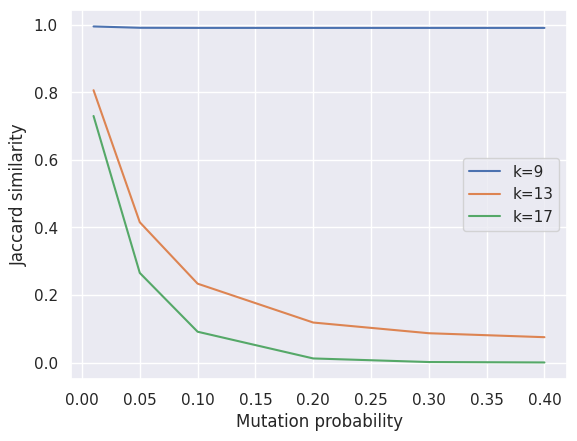
\includegraphics[width=0.8\textwidth]{jaccard}}
	
\subsection{}

Pozrime sa najskôr na prípad $k=9$. Vidíme, že by sme predpokladali, že pravdepodobnosť, že daný k-mer nájdeme v zmutovanom genóme by mala klesať a pri $40\%$ mutácii dosiahnuť iba približne $1\%$ avšak vidíme, že Jaccardova podobnosť ostáva aj napriek zvyšujúcej pravdepodobnosti okolo $99\%$. Toto je spôsobené tým, že počet rôznych 9-merov v našom skutočnom genóme 0 je $129821$ a teoretický maximálny počet rôznych 9-merov je $131072$ (máme $9$ pozícii na ktorých môžem byť jedna zo $4$ báz avšak každý 9-mer má svoj reverzný komplement a iba canonikly menší z nich sa dostane do výslednej množiny), čiže približne $99.05\%$, z čoho vyplýva, že aj úplne náhodná postupnosť báz rovnakej dĺžky ako náš genóm bude mať Jaccardovu podobnosť okolo $99\%$.
\\
\\
Teraz sa pozrime na prípad $k=17$, tu vidíme, že podobnosť klesá veľmi rýchlo a už pri $20\%$ mutácii je podobnosť blízka nulová, čiže od $20\%$ mutácii je náš zmutovaný genóm takmer nerozlíšiteľný od náhodného genómu pričom pri $40\%$ mutácii je už z pohľadu podobnosti úplne nerozlíšiteľný od náhodného. Preto je táto hodnota parametra $k$ je použiteľná iba pre gény o ktorých predpokladáme, že budú veľmi podobné.
\\
\\
Nakoniec zhodnoťme prípad $k=13$. Tu vidíme, že podobnosť postupne klesá (narozdiel od $k=9$) avšak pokles nie je veľmi rýchly (narozdiel od $k=17$) preto je táto hodnota zo všetkých troch najvhodnejšia na analýzu podobnosti.

\section{Task 5}

Ak vypočítame Jaccardovu podobnosť nášho skutočného genómu 0 s ostatným genómmi (aj sebou samým) použitím 13-merov dostaneme takéto hodnoty podobnosti: 
 
\begin{table}[!h]
	\begin{tabular}{|l|l|l|l|l|l|l|l|l|l|}
		\hline
		genóm  & 0 & 1 & 2 & 3 & 4 & 5 & 6 & 7 & 8  \\ \hline
		0 & 1.0 &
		0.6436 &
		0.2873 &
		0.0625 &
		0.1543 &
		0.5887 &
		0.1582 &
		0.1546 &
		0.1558 \\ \hline
		
	\end{tabular}
\end{table}

Vidíme, že najväčšiu podobnosť mám genóm 0 s genómmi 1 a 5 (samozrejme aj sebou samým ale to nie je zaujímavé). Táto podobnosť bola však aj predpokladateľná, keďže všetky 3 genómy sú genómmi baktérie s názvom Escherichia coli pričom vo všetkých troch prípadoch ide o kompletné genómy.

Keďže ide o genómy jedného druhu baktérie môžeme predpokladať, že rozdiely medzi nimi sú spôsobené hlavne náhodnými mutáciami. Ak sa pozrieme do tabuľky (a grafu) v úlohe 4 na riadok pre $k=13$ (krivku pre $k=13$) vidíme, že obe naše najpodobnejšie genómy majú hodnotu Jaccardovej podobnosti medzi hodnoty podobnosti pre pravdepodobnosť mutácie $1\%$ a $5\%$, pričom obe sú približne v strede tohto intervalu preto náš odhad je, že ak sú všetky rozdiely medzi genómom 0 a genómmi 1 a 5 spôsobené náhodnými mutáciami tak majú obe zmutovaných približne $3\%$ báz oproti genómu 0.  

\section{Task 6} 

\subsection{}

Ak na zmutované genómy použijeme funkciu minimizer s oknami veľkosti $w=2,5,10$ dostaneme takéto odhady Jaccardovej podobnosti:

\begin{table}[!h]
	\begin{tabular}{|l|l|l|l|l|l|l|}
		\hline
		w\textbackslash p & 0.01   & 0.05   & 0.1    & 0.2    & 0.3    & 0.4   \\ \hline
		2 & 0.7972 & 0.3987 & 0.2162 & 0.1033 & 0.0737 & 0.0633 \\ \hline
		5 & 0.7862 & 0.3774 & 0.1968 & 0.0897 & 0.0631 & 0.0539 \\ \hline
		10 & 0.773 & 0.3563 & 0.1826 & 0.083 & 0.0585 & 0.0505 \\ \hline
		
	\end{tabular}
\end{table}

Ak na tieto genómy použijeme namiesto funkcie minimizer funkciu minHash s veľkosťou výslednej množiny $m=10,100,1000$ dostaneme takéto odhady Jaccardovej podobnosti: 

\begin{table}[!h]
	\begin{tabular}{|l|l|l|l|l|l|l|}
		\hline
		m\textbackslash p & 0.01   & 0.05   & 0.1    & 0.2    & 0.3    & 0.4   \\ \hline
		10 &0.8 &0.5 &0.4 &0.2 &0.1 &0.1 \\ \hline
		100 &0.88 &0.6 &0.4 &0.25 &0.18 &0.17 \\ \hline
		1000 &0.895 &0.595 &0.377 &0.212 &0.148 &0.139 \\ \hline
		
	\end{tabular}
\end{table}

\subsection{}

Po vypočítaní rozdielu medzi Jaccardovou podobnosťou vypočítanou z všetkých k-merov a hodnotami získanými pomocou zmenšenej množiny pomocou metódy minimizer dostaneme takéto hodnoty:

\begin{table}[!h]
	\begin{tabular}{|l|l|l|l|l|l|l|}
		\hline
		w\textbackslash p & 0.01   & 0.05   & 0.1    & 0.2    & 0.3    & 0.4   \\ \hline
		2 & 0.0067 & 0.0157 & 0.0171 & 0.0153 & 0.0132 & 0.0119 \\ \hline
		5 & 0.0178 & 0.0371 & 0.0365 & 0.029 & 0.0238 & 0.0213 \\ \hline
		10 & 0.031 & 0.0582 & 0.0507 & 0.0357 & 0.0284 & 0.0247 \\ \hline
		
	\end{tabular}
\end{table}

Rozdiely medzi Jaccardovov podobnosťou vypočítanou z všetkých k-merov a hodnotami získanými pomocou zmenšenej množiny pomocou metódy miniHash sú následovné:
 

\begin{table}[!h]
	\begin{tabular}{|l|l|l|l|l|l|l|}
		\hline
		m\textbackslash p & 0.01   & 0.05   & 0.1    & 0.2    & 0.3    & 0.4   \\ \hline
		10 & 0.004 & -0.0855 & -0.1667 & -0.0814 & -0.0131 & -0.0248 \\ \hline
		100 & -0.076 & -0.1855 & -0.1667 & -0.1314 & -0.0931 & -0.0948 \\ \hline
		1000 & -0.091 & -0.1805 & -0.1437 & -0.0934 & -0.0611 & -0.0638 \\ \hline
		
	\end{tabular}
\end{table}

\subsection{}
Graf absolútnych hodnôt rozdielov odhadov Jaccardových podobností získaných zmenšením množiny k-mer pomocou metód minimizer a minHash s rôznymi hodnotami vstupných parametrov. 
\centerline{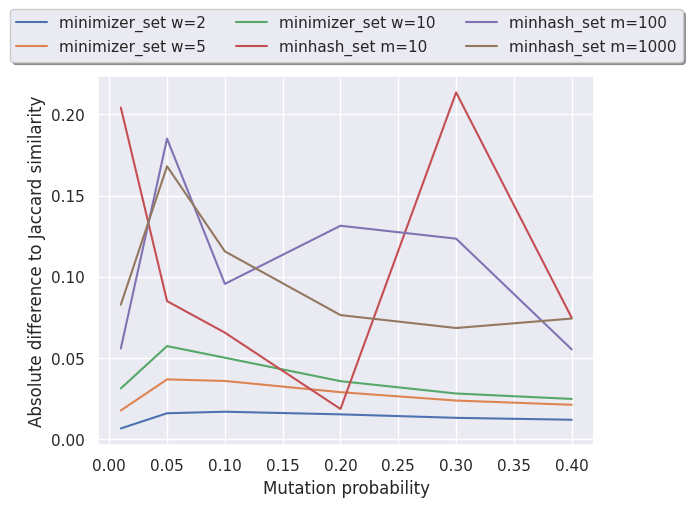
\includegraphics[width=0.8\textwidth]{download}}
\subsection{}

Vidíme, že ak množiny k-merov ktoré porovnávame získame metódou minimizer tak výsledná Jaccardova podobnosť je vo všeobecnosti menšia ako podobnosť získaná všetkými k-mermi. Zároveň môžeme vidieť, že rozdiely sú najmenšie pre okná veľkosti 2 ($w=2$) a so zväčšujúcou sa veľkosťou okna sa rozdiely zväčšujú čo je očakávané keďže so zväčšujúcim oknom odstraňuje stále viac a viac k-merov keďže k-mer s malou hodnotou hash bude patriť do viac okien a tým pádom bude vybraný viackrát avšak vo finálnej množine bude iba raz.
\\
\\
Pri porovnávaní hodnôt Jaccardovej podobnosti zo všetkých k-merov a podmnožiny vybranej pomocou metódy minHash si môžeme všimnúť, že narozdiel od metódy minimizer sú tieto hodnoty podobnosti vo všeobecne nadhodnotené (väčšie ako hodnota získaná zo všetkých k-merov). Predpokladali by sme, že so zväčšujúcou množinou vybraných k-merov by sa odhadnutá podobnosti mala stále viac približovať hodnota získanej zo všetkých k-merov, avšak z nejakého dôvodu sa mi v tomto prípade tento predpoklad nepotvrdil keď najlepšie odhady boli pre množinu veľkosti 10 ($m=10$) a pre obe väčšie množiny dostávame veľmi podobné rozdiely.
\\
\\
Ak porovnáme vzájomne výsledky oboch metód môžeme si všimnúť, že metóda minimizer má výrazne menšie chyby ako metóda minHash (viď graf v 6.3).

\section{Task 7} 

\subsection{}
\subsection{}
\subsection{}
Tabuľka časov výpočtu a veľkostí výsledných množín.
\begin{table}[!h]
	\begin{tabular}{|l|l|l|l|l|l|l|l|}
		\hline
		funkcia  & full\_kmer\_set  & \multicolumn{3}{|l|}{minimizer\_set}   & \multicolumn{3}{|l|}{minihash\_set}   \\ \hline
		parameter & -  & w=2   & w=5    & w=10    & m=10   & m=100 & m=1000   \\ \hline
		čas (s) & 19.51 & 45.01 & 45.21 & 48.99 & 39.08 & 38.82 & 38.54\\ \hline
		priestor & 3,852,750 & 2,629,171 & 1,341,096 & 736,529 & 10 & 100 & 1000 \\ \hline
	\end{tabular}
\end{table}

\subsection{}

\subsection{}
V tabuľke môžeme vidieť, že metóda full\_kmer\_set je jednoznačne najrýchlejšia (čo je samozrejme spôsobené aj tým, že obe ďalšie metódy musia počas svojho chodu vypočítať postupne všetky k-mery z ktorých postupne vyberajú výsledné) avšak časy zvyšných metód sú len niečo vyše dvojnásobné čo by mohlo indikovať, že ich reálna výpočtová zložitosť je väčšia iba o konštantný násobok. Táto metódy má však najväčšiu priestorovú zložitosť, keďže výsledná množina obsahuje všetky rôzne k-mery ktoré sa v genóme vyskytujú zatiaľ čo zvyšné metódy obsahujú iba akúsi ich podmnožinu.
\\
\\
V prípade časov metódy minimizer\_set si môžeme všimnúť, že zo zväčšujúcim sa oknom sa doba výpočtu mierne predlžuje, tento výsledok by sme mohli vysvetliť tým, čím máme väčšie okno tým dlhšie trvá hľadanie najmenšej hodnoty hash k-merov v ňom. Z pohľadu priestorovej zložitosť vidíme výrazný pokles kedy už pri okne veľkosti $w=2$ klesol počet len na približne $70\%$ a pri okne veľkosti $w=10$ výsledná množina obsahuje iba približne $20\%$ pôvodnej množiny.
\\
\\
Ak sa pozrieme na výsledky metódy minhash\_set môžeme vidieť, že zväčšujúcou hodnotou $m$ sa časy skracujú čo je minimálne pre mňa prekvapujúce keďže bez ohľadu na hodnotu $m$ musí prejsť cez všetky k-mery a zo zväčšujúcou hodnotou $m$ by sa mala zväčšovať zložitosť vkladania a výberu z prioritnej fronty ktorú využívame na ukladanie k-merov s priebežne najmenšou hash hodnotou. Priestorová zložitosť je presne taká ako by sme očakávali keďže je priamo určená vstupným parametrom $m$.
\\
\\
Keď vezmeme do úvahy výsledky z Task 6 a Task 7, tak jednoznačne ak výrazne obmedzený priestor s ktorým vieme pracovať tak aj napriek pomerne veľkým chybám v odhadoch je najvhodnejšie použiť minHash metódu na zmenšenie množiny k-merov na konkrétnu veľkosť (alternatívou môže byť aj použitie metódy minimizer s pomerne veľkým oknom).
Ak šetrenie priestoru nie je prioritou tak metóda minimizer si síce vyžiada približne dvojnásobný čas na vytvorenie množiny k-merov ale výsledná množina je výrazne menšia ako množina všetkých k-merov vďaka čomu je výpočet Jaccardovej podobnosti rýchlejší pričom chyba tejto podobnosti v porovnaní s podobnosťou s použitím celej množiny je pomerne malá.
Preto moje odporúčanie by bolo použitie metódy minimizer s veľkosťou okna okolo 5 čím zmenšíme množinu k-merov na menej ako polovicu ale stále dostaneme pomerne blízke výsledky.

\end{document}
